\subsection{Простейшее XOR-шифрование}

Однажды я видел ПО, где все отладочные сообщения были зашифрованы используя XOR со значением 3.
Иными словами, 2 младших бита каждого символа были переключены.

``Hello, world'' становилось ``Kfool/\#tlqog'':

\begin{lstlisting}[caption=Python,style=custompy]
#!/usr/bin/python

msg="Hello, world!"

print "".join(map(lambda x: chr(ord(x)^3), msg))
\end{lstlisting}

Это интересное шифрование (или даже обфускация), потому что оно имеет два важных свойства:
1) одна ф-ция для шифрования/дешифрования, просто вызовите её еще раз;
2) символы на выходе печатаемые, так что вся строка может быть использована в исходном коде без специальных (\text{escaping}) символов.

Второе свойство использует тот факт что все печатаемые символы расположены в рядах: 0x2x-0x7x, и когда вы меняете
два младших бита, символ \emph{перемещается} на 1 или 3 символа влево или вправо, но никогда не \emph{перемещается} в другой
(может быть, непечатаемый) ряд:

\begin{figure}[H]
\centering
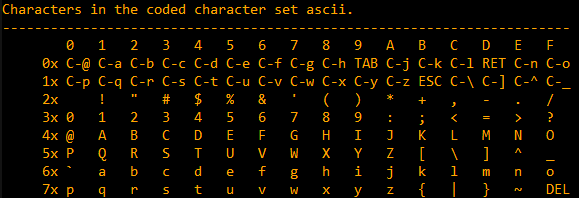
\includegraphics[width=0.8\textwidth]{ascii_clean.png}
\caption{7-битная \ac{ASCII}-таблица в Emacs}
\end{figure}

\dots с единственным исключением символа 0x7F.

Например, давайте \emph{зашифруем} символы в пределах A-Z:

\begin{lstlisting}
#!/usr/bin/python

msg="@ABCDEFGHIJKLMNO"

print "".join(map(lambda x: chr(ord(x)^3), msg))
\end{lstlisting}

Результат: \verb|CBA@GFEDKJIHONML|.

Это как если символы ``@'' и ``C'' были поменены местами, и так же и ``B'' и ``a''.

Так или иначе, это интересный пример использующий свойства XOR, нежели шифрование:
тот самый эффект \emph{сохранения печатаемости} может быть достигнут переключая любой из младших 4-х бит,
в любой последовательности.

